%-------------------------------------------------------------------------------------------------------------------------------%
%*******************************************************************************************************************************%
%************************************************** Dissertation-Schultze.tex **************************************************%
%*******************************************************************************************************************************%
%-------------------------------------------------------------------------------------------------------------------------------%
\documentclass{thesis}
%-------------------------------------------------------------------------------------------------------------------------------%
% thesis.tex included packages
\usepackage{epsfig}                 %% Permit the use of postscript figures within the document.
%\patchcmd{\Ginclude@eps}{"#1"}{#1}{}{}
%\usepackage{chicago}                %% Use chicago style bibliography
%\bibliographystyle{chicago}
%\bibliographystyle{IEEEtran}
%-------------------------------------------------------------------------------------------------------------------------------%
%*******************************************************************************************************************************%
%************************************************** Dissertation-Preamble.tex **************************************************%
%*******************************************************************************************************************************%
%-------------------------------------------------------------------------------------------------------------------------------%
\makeatletter
%-------------------------------------------------------------------------------------------------------------------------------%
%~~~~~~~~~~~~~~~~~~~~~~~~~~~~~~~~~~~~~~~~~~~~~~~~~~~~~~~~~~~~~~~~~~~~~~~~~~~~~~~~~~~~~~~~~~~~~~~~~~~~~~~~~~~~~~~~~~~~~~~~~~~~~~~%
%~~~~~~~~~~~~~~~~~~~~~~~~~~~~~~~~~~~~~ Dissertation Specific Control Sequence Definitions ~~~~~~~~~~~~~~~~~~~~~~~~~~~~~~~~~~~~~~%
%~~~~~~~~~~~~~~~~~~~~~~~~~~~~~~~~~~~~~~~~~~~~~~~~~~~~~~~~~~~~~~~~~~~~~~~~~~~~~~~~~~~~~~~~~~~~~~~~~~~~~~~~~~~~~~~~~~~~~~~~~~~~~~~%
%-------------------------------------------------------------------------------------------------------------------------------%
% Uncomment if topics are presented as Chapters
\def\partition{Chapter}
\def\partitions{Chapters}
\def\subpartition{Section}
\def\subpartitions{Sections}
\def\subsubpartition{Subsection}
\def\subsubpartitions{Subsections}
%\def\commonMethods{Chapter~\ref{chap:methods}}
\def\commonMethods{Chapter~\ref{chap:methods} (Methods)}
\def\reftag{chap}
%-------------------------------------------------------------------------------------------------------------------------------%
%% Uncomment if topics are presented as Sections of Chapter 3: Methods
%\def\partition{Section}
%\def\partitions{Sections}
%\def\subpartition{Subsection}
%\def\subpartitions{Subsections}
%\def\subsubpartition{Subsubsection}
%\def\subsubpartitions{Subsubsections}
%%\def\commonMethods{the introduction of Chapter~\ref{chap:methods}}
%\def\commonMethods{the introduction of Chapter~\ref{chap:methods} (Methods)}
%\def\reftag{sec}
%-------------------------------------------------------------------------------------------------------------------------------%
\def\pix{\mathcal{P}}
\def\L{{\mathcal{L}}}
\def\VL{{\vect{\mathcal{L}}}}
\def\I{\mathcal{I}}
\def\xray{x-ray}
\def\xrays{x-rays}
\def\xCT{x-ray CT}
\def\WEPL{water-equivalent path length}
\def\WET{water-equivalent thickness}
\def\iiSCuts{$2\sigma$~cuts}
\def\iiSWCuts{$2\sigma$~WEPL cuts}
\def\iiSACuts{$2\sigma$~scattering angle cuts}
\def\iiSWACuts{$2\sigma$~WEPL and scattering angle cuts}
\def\arrowsym{\rightharpoonup}%
\def\vectfill{$\raisebox{-0.0pt}[\p@][\p@]{\upshape$\vstretch{1}{\scaleobj{1}{\arrowsym}}$}$}
%-------------------------------------------------------------------------------------------------------------------------------%
\newcommand{\CatphanTM}{{Catphan\textsuperscript{\textregistered}}}
\newcommand{\CTP}{{CTP404\space}}
\newcommand{\CatphanTMlong}{{\CatphanTM}\space\CTP}
\newcommand{\npclass}{$\cal{NP}$}
%-------------------------------------------------------------------------------------------------------------------------------%
%*******************************************************************************************************************************%
%************************************************ END: Dissertation-Preamble.tex ***********************************************%
%*******************************************************************************************************************************%
%-------------------------------------------------------------------------------------------------------------------------------%
\makeatother
\endinput
%%-------------------------------------------------------------------------------------------------------------------------------%
     %% Additional packages and other preamble content (defs, commands, etc.)
%_______________________________________________________________________________________________________________________________%
%*******************************************************************************************************************************%
%===============================================================================================================================%
%-------------------------------------------------- Dissertation-Prologue.tex --------------------------------------------------%
%===============================================================================================================================%
%*******************************************************************************************************************************%
% File: Dissertation-Prologue.tex
% Description: this file is where the abstract, acknowledgements, dedication, and attributions should be defined AND/OR excluded.
% Usage: + Fill in the \X{...} macros that you want to be INCLUDED in your document; this automatically sets the corresponding
%        \if@makeXPage conditional to TRUE and inserts the associated \thesisXPage into the document in the proper order.     
%        + To EXCLUDE any of these frontmatter pages from the document, uncomment the corresponding \excludeX macros. Commenting
%        out the \X{...} macro will also prevent the corresponding Page from being included in the document.
%
%
%_______________________________________________________________________________________________________________________________%
% Last Updated in December, 2023
%_______________________________________________________________________________________________________________________________%
%===============================================================================================================================%
%------------------------------------------------------ Prologue Controls ------------------------------------------------------%
%===============================================================================================================================%
%\makeCopyrightPage
%\makeListOfFigures
%\makeListOfTables
%-------------------------------------------------------------------------------------------------------------------------------%
%\excludeAbstractPage
%\excludeAcknowlegmentsPage
%\excludeDedicationPage
%\excludeAttributionsPage
%\emptyLoT                                                              % Tell latex that there is no list of tables
%-------------------------------------------------------------------------------------------------------------------------------%
%\setUppercaseHeadings
%\setCapitalizedHeadings
%-------------------------------------------------------------------------------------------------------------------------------%
%\setUppercaseToCtitles
%\setCapitalizedToCtitles
%-------------------------------------------------------------------------------------------------------------------------------%
%\setLoZtitlesAligned
%\setLoZtitlesConstsep
%-------------------------------------------------------------------------------------------------------------------------------%
%\cftsetindents{figure}{0in}{\len@p@figure}                                      % Increase the width of the figure number line box to contain "Figure X.XX", but reduce the gap before subsequent title by 1em to ~1 space DEFAULT:{1.5em}{2.3em}
%\cftsetindents{table}{0in}{\len@p@table}                                        % Increase the width of the table number line box to contain "Table X.XX", but reduce the gap before subsequent title by 1em to ~1 space DEFAULT:{1.5em}{2.3em}
%\cftsetindents{chapter}{0in}{0in}
%\cftsetindents{section}{\cftindent@between@chap@sec}{0in}
%\cftsetindents{subsection}{\cftindent@between@chaplines+\cftindent@between@any@sec*2}{0in}
%\cftsetindents{subsubsection}{\cftindent@between@chaplines+\cftindent@between@any@sec*3}{0in}
%\cftsetindents{paragraph}{\cftindent@between@chaplines+\cftindent@between@any@sec*4}{0in}
%_______________________________________________________________________________________________________________________________%
%*******************************************************************************************************************************%
%===============================================================================================================================%
%--------------------------------------------------------- FRONTMATTER ---------------------------------------------------------%
%-------------------------------------------------------------------------------------------------------------------------------%
%----------------------------------------- Frontmatter (Prologue) page(s) text content -----------------------------------------%
%===============================================================================================================================%
%*******************************************************************************************************************************%
%_______________________________________________________________________________________________________________________________%
%===============================================================================================================================%
%---------------------------------------------------------- Abstract -----------------------------------------------------------%
%===============================================================================================================================%
\abstract{The work presented in this dissertation...
}
%===============================================================================================================================%
%------------------------------------------------------ Acknowledgements -------------------------------------------------------%
%===============================================================================================================================%
\acknowledgements{Special thanks go to...
}
%===============================================================================================================================%
%--------------------------------------------------------- Dedication ----------------------------------------------------------%
%===============================================================================================================================%
%-------------------------------------------------------------------------------------------------------------------------------%
%\setDedicationFontstyle{it}
%\setPageFontstyle{Dedication}{bf}
%-------------------------------------------------------------------------------------------------------------------------------%
\dedication{This is dedicated to...
}
%===============================================================================================================================%
%-------------------------------------------------------- Attributions ---------------------------------------------------------%
%===============================================================================================================================%
%-------------------------------------------------------------------------------------------------------------------------------%
% Example usage of the \attributions macro and the associated 'attributionList', 'attribution', and 'authorList' environments
% designed to generate an appropriately formatted attributions list.
%-------------------------------------------------------------------------------------------------------------------------------%
\attributions{%
\begin{attributionList}
%-------------------------------------------------------------------------------------------------------------------------------%
    \item\begin{attribution}
        %Schultze, B. E., M. Witt, Y. Censor, K. E. Schubert, and R. W. Schulte (2015). Performance of hull-detection algorithms for proton computed tomography reconstruction. In S. Reich and A. Zaslavski (Eds.), \textit{Infinite Products of Operators and Their Applications}, Volume 636 of \textit{Contemporary Mathematics}, pp. 211–224. American Mathematical Society.
         B. E. Schultze, M. Witt, Y. Censor, K. E. Schubert, and R. W. Schulte, “Performance of hull-detection algorithms for proton computed tomography reconstruction,” in \textit{Infinite Products of Operators and Their Applications}, ser. Contemporary Mathematics, S. Reich and A. Zaslavski, Eds., vol. 636. American Mathematical Society, 2015, pp. 211–224.
    \end{attribution}\label{attribution:hull-detection}%
    \begin{authorList}
        \item I (B. E. Schultze) was the sole investigator and primary author of the publication.
        \item M. Witt provided the simulated data sets used for the initial hull-detection investigations.
        \item Y. Censor, K. E. Schubert, and R. W. Schulte acted in a supervisory role on editing, content accuracy, and approval of the final form submitted for publication.
    \end{authorList}
%-------------------------------------------------------------------------------------------------------------------------------%
    \item\begin{attribution}%
        %Schultze, B. E., Y. Censor, P. Karbasi, K. E. Schubert, and R. W. Schulte (2020). An Improved Method of Total Variation Superiorization Applied to Reconstruction in Proton Computed Tomography. \textit{IEEE Transactions on Medical Imaging 39}(2), 294–307.
        B. E. Schultze, Y. Censor, P. Karbasi, K. E. Schubert, and R. W. Schulte, “An Improved Method of Total Variation Superiorization Applied to Reconstruction in Proton Computed Tomography,” \textit{IEEE Transactions on Medical Imaging}, vol. 39, no. 2, pp. 294–307, 2020
    \end{attribution}\label{attribution:ntvs}
    \begin{authorList}
        \item I (B. E. Schultze) was the sole investigator and primary author of the publication.
        \item Y. Censor is among the original developers of the superiorization methodology, which serves as the theoretical framework of total variation superiorization, and requested the investigations be performed for pCT. He also provided approval of the investigation results and final form submitted for publication.
        \item P. Karbasi was a colleague working independently on a related topic who participated in discussions to ensure our investigations did not overlap. She also assisted in the editing of the final form submitted for publication.
        \item K. E. Schubert and R. W. Schulte acted in a supervisory role on editing, content accuracy, and approval of the final form submitted for publication.%
    \end{authorList}%
\end{attributionList}
}
%_______________________________________________________________________________________________________________________________%
%*******************************************************************************************************************************%
%===============================================================================================================================%
%----------------------------------------------- END: Dissertation-Prologue.tex ------------------------------------------------%
%===============================================================================================================================%
%*******************************************************************************************************************************%
\endinput

\graphicspath{{./images/}}
%-------------------------------------------------------------------------------------------------------------------------------%
%% One of the most important things you have to do in the preamble is
%% to tell who you are and what your thesis is about.
%%
%\newcommand*{\degree}[1]{\gdef\thesisDegree{#1}}
%\newcommand*{\supervisor}[1]{\gdef\thesisMentor{#1}}
%\newcommand*{\supervisorTitle}[1]{\gdef\thesisMentorTitle{#1}}
%\newcommand*{\seeking}[1]{\gdef\thesisSeeking{#1}}
%\newcommand*{\holding}[1]{\gdef\thesisHolding{#1}}
%\newcommand*{\readerOne}[1]{\gdef\thesisReaderOne{#1}}
%\newcommand*{\readerTwo}[1]{\gdef\thesisReaderTwo{#1}}
%\newcommand*{\department}[1]{\gdef\thesisDepartment{#1}}
%\newcommand*{\departmentChair}[1]{\gdef\thesisDepartmentChair{#1}}
%\newcommand*{\graduateDean}[1]{\gdef\thesisDean{#1}}
%\renewcommand*{\date}[1]{\gdef\thesisConfDate{#1}}
%\renewcommand*{\author}[1]{\gdef\thesisAuthorName{#1}}
%\renewcommand{\abstract}[1]{\gdef\thesisAbstract{#1}}
%
%% Optional parameters
%\newcommand*{\acknowledgements}[1]{\@makeAcknowledgementstrue \gdef\th@acknowledgementsStash{#1}}
%\newcommand{\dedication}[1]{\@makeDedicationtrue \gdef\th@dedicationStash{#1}}
%\newcommand*{\readerThree}[1]{\@makeReaderThreetrue \gdef\thesisReaderThree{#1}}
%\newcommand*{\readerFour}[1]{\@makeReaderFourtrue \gdef\thesisReaderFour{#1}}
%\newcommand*{\readerFive}[1]{\@makeReaderFivetrue \gdef\thesisReaderFive{#1}}
%\newcommand*{\makeListOfFigures}{\@makeLoFtrue}
%\newcommand*{\makeListOfTables}{\@makeLoTtrue}

\title{Essential Elements of Proton Computed Tomography for Practical Applications}%\thesisTitle

\author{Blake Edward Schultze}                                          %\thesisAuthor
\holding{B.S., M.S.}                                                          %\thesisHolding
\seeking{Ph.D.}                                                         %\thesisSeeking
\degree{Doctor of Philosophy}                                           %\thesisDegree

\department{Department of Electrical and Computer Engineering}          %\thesisDepartment
\departmentChair{Kwang Y. Lee, Ph.D.}                                   %\thesisDepartmentChair
%\schoolChair{Kwang Y. Lee, Ph.D.}
\graduateDean{J. Larry Lyon, Ph.D.}                                     %\thesisDean
\supervisor{Keith Evan Schubert, Ph.D.}                                 %\thesisMentor
\supervisorTitle{Mentor}                                                %\thesisMentorTitle
\readerOne{Robert J. Marks II, Ph.D.}                                   %\thesisReaderOne
\readerTwo{Jeffrey S. Olafson, Ph.D.}                                   %\thesisReaderTwo
\readerThree{Reinhard W. Schulte, Ph.D.}                                %\thesisReaderThree
\date{August 2021}                                                      %\thesisConfDate

%% You may have to change these but probably not.

\insertSignaturePage{./Forms/SignaturesPage-Schultze.pdf}
%\makeCopyrightPage
\makeListOfFigures                                                      % sets \@makeLoFtrue -> adds \thesisLoFpage to \thesisPrologue
\makeListOfTables                                                       % sets \@makeLoTtrue -> adds \thesisLoTpage to \thesisPrologue

% Tell latex that there is no list of tables
%\emptyLoT

%%-------------------------------------------------------------------------------------------------------------------------------%
%%~~~~~~~~~~~~~~~~~~~~~~~~~~~~~~~~~~~~~~~~~~~~~~~~~~~~~~~~~~~~~~~~~~~~~~~~~~~~~~~~~~~~~~~~~~~~~~~~~~~~~~~~~~~~~~~~~~~~~~~~~~~~~~~%
%%~~~~~~~~~~~~~~~~~~~~~~~~~~~~~~~~~~~~~~~~~~~~~~~~~~~~~~~~~~~ Abstract ~~~~~~~~~~~~~~~~~~~~~~~~~~~~~~~~~~~~~~~~~~~~~~~~~~~~~~~~~~%
%%~~~~~~~~~~~~~~~~~~~~~~~~~~~~~~~~~~~~~~~~~~~~~~~~~~~~~~~~~~~~~~~~~~~~~~~~~~~~~~~~~~~~~~~~~~~~~~~~~~~~~~~~~~~~~~~~~~~~~~~~~~~~~~~%
%%-------------------------------------------------------------------------------------------------------------------------------%
%\abstract{The work presented in this dissertation all pertains to developments of proton computed tomography (pCT) and the elements essential to its viability as a clinical imaging modality. This includes methodological and implementational developments for reducing reconstruction time and improving pCT image quality, each advancing pCT towards clinical viability. The corresponding methods are presented in the chronological order of their development.
%
%Hull-detection, a method for differentiating voxels internal and external to an object, is presented first. Hull-detection was specifically developed for pCT as a preferable means for obtaining a binary image of the object, a preconditioning step often referred to as object detection. The concept of hull-detection, similar to the way a sculptor chisels away portions of material to produce the desired sculpture, is that voxels along the paths of protons that completely miss the object can be carved away to reveal the object hull. However, this neglects to account for the ramifications of uncertainties in the data, which was accounted for in different ways. Several hull-detection algorithms were developed and compared to the classic object detection method based on thresholding the filtered backprojection image.
%
%The second topic presented is efficiently implementing the most-likely path (MLP) formalism for pCT. This formalism was developed to more accurately approximate proton paths within an object, increasing the achievable spatial resolution. Computing the MLP is, by far, the most computationally expensive task performed during image reconstruction, making it the biggest hurdle to achieving clinically viable image reconstruction times (below 10 minutes). A computationally efficient implementation of the MLP was developed by simplifying the associated equations and incorporating several software design principles to reduce the number of compute operations and improve numerical stability.
%
%The final topic presented is the incorporation of recent advancements of total variation superiorization (TVS) into pCT. A fixed parameter version of TVS was initially incorporated into the feasibility-seeking algorithms of pCT, which included a step verifying successful TV reduction. Presented here is the modern version of TVS applied to pCT, with user-control of parameters, removal of the verification step, and additional option to perform repeated perturbations.
%}
%%-------------------------------------------------------------------------------------------------------------------------------%
%%~~~~~~~~~~~~~~~~~~~~~~~~~~~~~~~~~~~~~~~~~~~~~~~~~~~~~~~~~~~~~~~~~~~~~~~~~~~~~~~~~~~~~~~~~~~~~~~~~~~~~~~~~~~~~~~~~~~~~~~~~~~~~~~%
%%~~~~~~~~~~~~~~~~~~~~~~~~~~~~~~~~~~~~~~~~~~~~~~~~~~~~~~~ Acknowledgements ~~~~~~~~~~~~~~~~~~~~~~~~~~~~~~~~~~~~~~~~~~~~~~~~~~~~~~%
%%~~~~~~~~~~~~~~~~~~~~~~~~~~~~~~~~~~~~~~~~~~~~~~~~~~~~~~~~~~~~~~~~~~~~~~~~~~~~~~~~~~~~~~~~~~~~~~~~~~~~~~~~~~~~~~~~~~~~~~~~~~~~~~~%
%%-------------------------------------------------------------------------------------------------------------------------------%
%\acknowledgements{Special thanks go to my long term mentor, Dr. Keith Schubert, and his wife Kym Schubert for their support throughout my academic journey. I would also like to thank my fellow Baylor student colleagues, professors, and support staff for their roles in my success, particularly Minnie Simcik, Brian Sitton, Pat Hynan, Kay Riddering, Robert Marks III, Paniz Karbasi, and Ritchie Cai. I would also like to extend my gratitude to those at CSUSB that offered guidance and support along the way, particularly Dr. Paul K. Dixon, Dr. Laura Woodney, and Dr. Ernesto Gomez.
%
%Additional thanks go out to the pCT Collaboration and its members for their contributions to and support of my research; in particular, I would like to thank Reinhard W. Schulte, Vladimir A. Bashkirov, Yair Censor, Ford Hurley, Valentina Giacommetti, Christina Sarosiek, George Coutrakon, and Robert P. Johnson.%\protect\noexpand\par}%
%
%The research in proton CT presented in this dissertation was supported by the National Institute of Biomedical Imaging and Bioengineering (NIBIB) of the National Institute of Health (NIH) and the National Science Foundation (NSF) award number~R01EB013118, and the United States - Israel Binational Science Foundation (BSF) grants no. 2009012 and no. 2013003. The content of this paper is solely the responsibility of Blake Edward Schultze and does not necessarily represent the official views of NBIB, NIH, or BSF.  The support of UT Southwestern and State of Texas through a Seed Grants in Particle Therapy award is also gratefully acknowledged.
%}
%%-------------------------------------------------------------------------------------------------------------------------------%
%%~~~~~~~~~~~~~~~~~~~~~~~~~~~~~~~~~~~~~~~~~~~~~~~~~~~~~~~~~~~~~~~~~~~~~~~~~~~~~~~~~~~~~~~~~~~~~~~~~~~~~~~~~~~~~~~~~~~~~~~~~~~~~~~%
%%~~~~~~~~~~~~~~~~~~~~~~~~~~~~~~~~~~~~~~~~~~~~~~~~~~~~~~~~ Attributions ~~~~~~~~~~~~~~~~~~~~~~~~~~~~~~~~~~~~~~~~~~~~~~~~~~~~~~~~~%
%%~~~~~~~~~~~~~~~~~~~~~~~~~~~~~~~~~~~~~~~~~~~~~~~~~~~~~~~~~~~~~~~~~~~~~~~~~~~~~~~~~~~~~~~~~~~~~~~~~~~~~~~~~~~~~~~~~~~~~~~~~~~~~~~%
%%-------------------------------------------------------------------------------------------------------------------------------%
%\attributions{%
%\begin{enumerate}[topsep=0pt, itemsep=0pt]%
%\item\begin{singlespace}%
%%Schultze, B. E., M. Witt, Y. Censor, K. E. Schubert, and R. W. Schulte (2015). Performance of hull-detection algorithms for proton computed tomography reconstruction. In S. Reich and A. Zaslavski (Eds.), \textit{Infinite Products of Operators and Their Applications}, Volume 636 of \textit{Contemporary Mathematics}, pp. 211–224. American Mathematical Society.
% B. E. Schultze, M. Witt, Y. Censor, K. E. Schubert, and R. W. Schulte, “Performance of hull-detection algorithms for proton computed tomography reconstruction,” in \textit{Infinite Products of Operators and Their Applications}, ser. Contemporary Mathematics, S. Reich and A. Zaslavski, Eds., vol. 636. American Mathematical Society, 2015, pp. 211–224.
%\end{singlespace}%
%\begin{itemize}[topsep=0pt,itemsep=0pt]%
%\item I (B. E. Schultze) was the sole investigator and author of the publication.
%\item M. Witt provided the simulated data sets used for the initial hull-detection investigations.
%\item Y. Censor, K. E. Schubert, and R. W. Schulte acted in a supervisory role on editing, content accuracy, and approval of the final form submitted for publication.
%\end{itemize}%
%%\vspace{0.25em}
%%\noindent where I (B. E. Schultze) was the primary investigator and author, M. Witt provided the simulated data sets used for hull-detection investigations, and Y. Censor, K. E. Schubert, and R. W. Schulte acted in a supervisory role on editing, content accuracy, and approval of the final form submitted for publication.
%\item\begin{singlespace}%
%%Schultze, B. E., Y. Censor, P. Karbasi, K. E. Schubert, and R. W. Schulte (2020). An Improved Method of Total Variation Superiorization Applied to Reconstruction in Proton Computed Tomography. \textit{IEEE Transactions on Medical Imaging 39}(2), 294–307.
%B. E. Schultze, Y. Censor, P. Karbasi, K. E. Schubert, and R. W. Schulte, “An Improved Method of Total Variation Superiorization Applied to Reconstruction in Proton Computed Tomography,” \textit{IEEE Transactions on Medical Imaging}, vol. 39, no. 2, pp. 294–307, 2020
%\end{singlespace}%
%\begin{itemize}[topsep=0pt,itemsep=0pt]%
%\item I (B. E. Schultze) was the sole investigator and author of the publication.
%\item Y. Censor is among the original developers of the superiorization methodology, which serves as the theoretical framework of total variation superiorization, and requested the investigations be performed for pCT. He also provided approval of the investigation results and final form submitted for publication.
%\item P. Karbasi was a colleague working independently on a related topic who participated in discussions to ensure our investigations did not overlap. She also assisted in the editing of the final form submitted for publication.
%\item K. E. Schubert and R. W. Schulte acted in a supervisory role on editing, content accuracy, and approval of the final form submitted for publication.
%\end{itemize}
%%\vspace{0.25em}
%%\noindent where I (B. E. Schultze) was the primary investigator and author, Y. Censor is among the original developers of the theoretical framework of TVS and was the person that requested and approved the TVS investigations, P. Karbasi was a colleague working independently on a related topic that helped to ensure our investigations did not overlap as well as assisted in editing, and K. E. Schubert and R. W. Schulte acted in a supervisory role on editing, content accuracy, and approval of the final form submitted for publication.
%\end{enumerate}
%}
%-------------------------------------------------------------------------------------------------------------------------------%
%*******************************************************************************************************************************%
%****************************************************** MAIN DOCUMENT BODY *****************************************************%
%*******************************************************************************************************************************%
%-------------------------------------------------------------------------------------------------------------------------------%
%    \nobibliography*    % Read in .bbl file entries for in text \bibentry citations, but also create back matter Bibliography
\begin{document}
	
%\include{C1-Intro-Attributed}
\include{C1-Intro-NotAttributed}

%_______________________________________________________________________________________________________________________________%
%*******************************************************************************************************************************%
%===============================================================================================================================%
%--------------------------------------------------- C2-HistoricalReview.tex ---------------------------------------------------%
%===============================================================================================================================%
%*******************************************************************************************************************************%
%_______________________________________________________________________________________________________________________________%
%-------------------------------------------------------------------------------------------------------------------------------%
\chapter{Historical Review and Literature Survey}\label{chap:history}

Present history of the research in your field/topic and an overview of the published literature relevant to this work. Prove that you are knowledgable about the existing literature in your field/topic so you can show why what you have done truly is new and important and represents a worthwhile contribution to the advancement of this field/topic.

\textbf{NOTE:} This may be broken into two chapters.
\begin{figure}
    \centering
    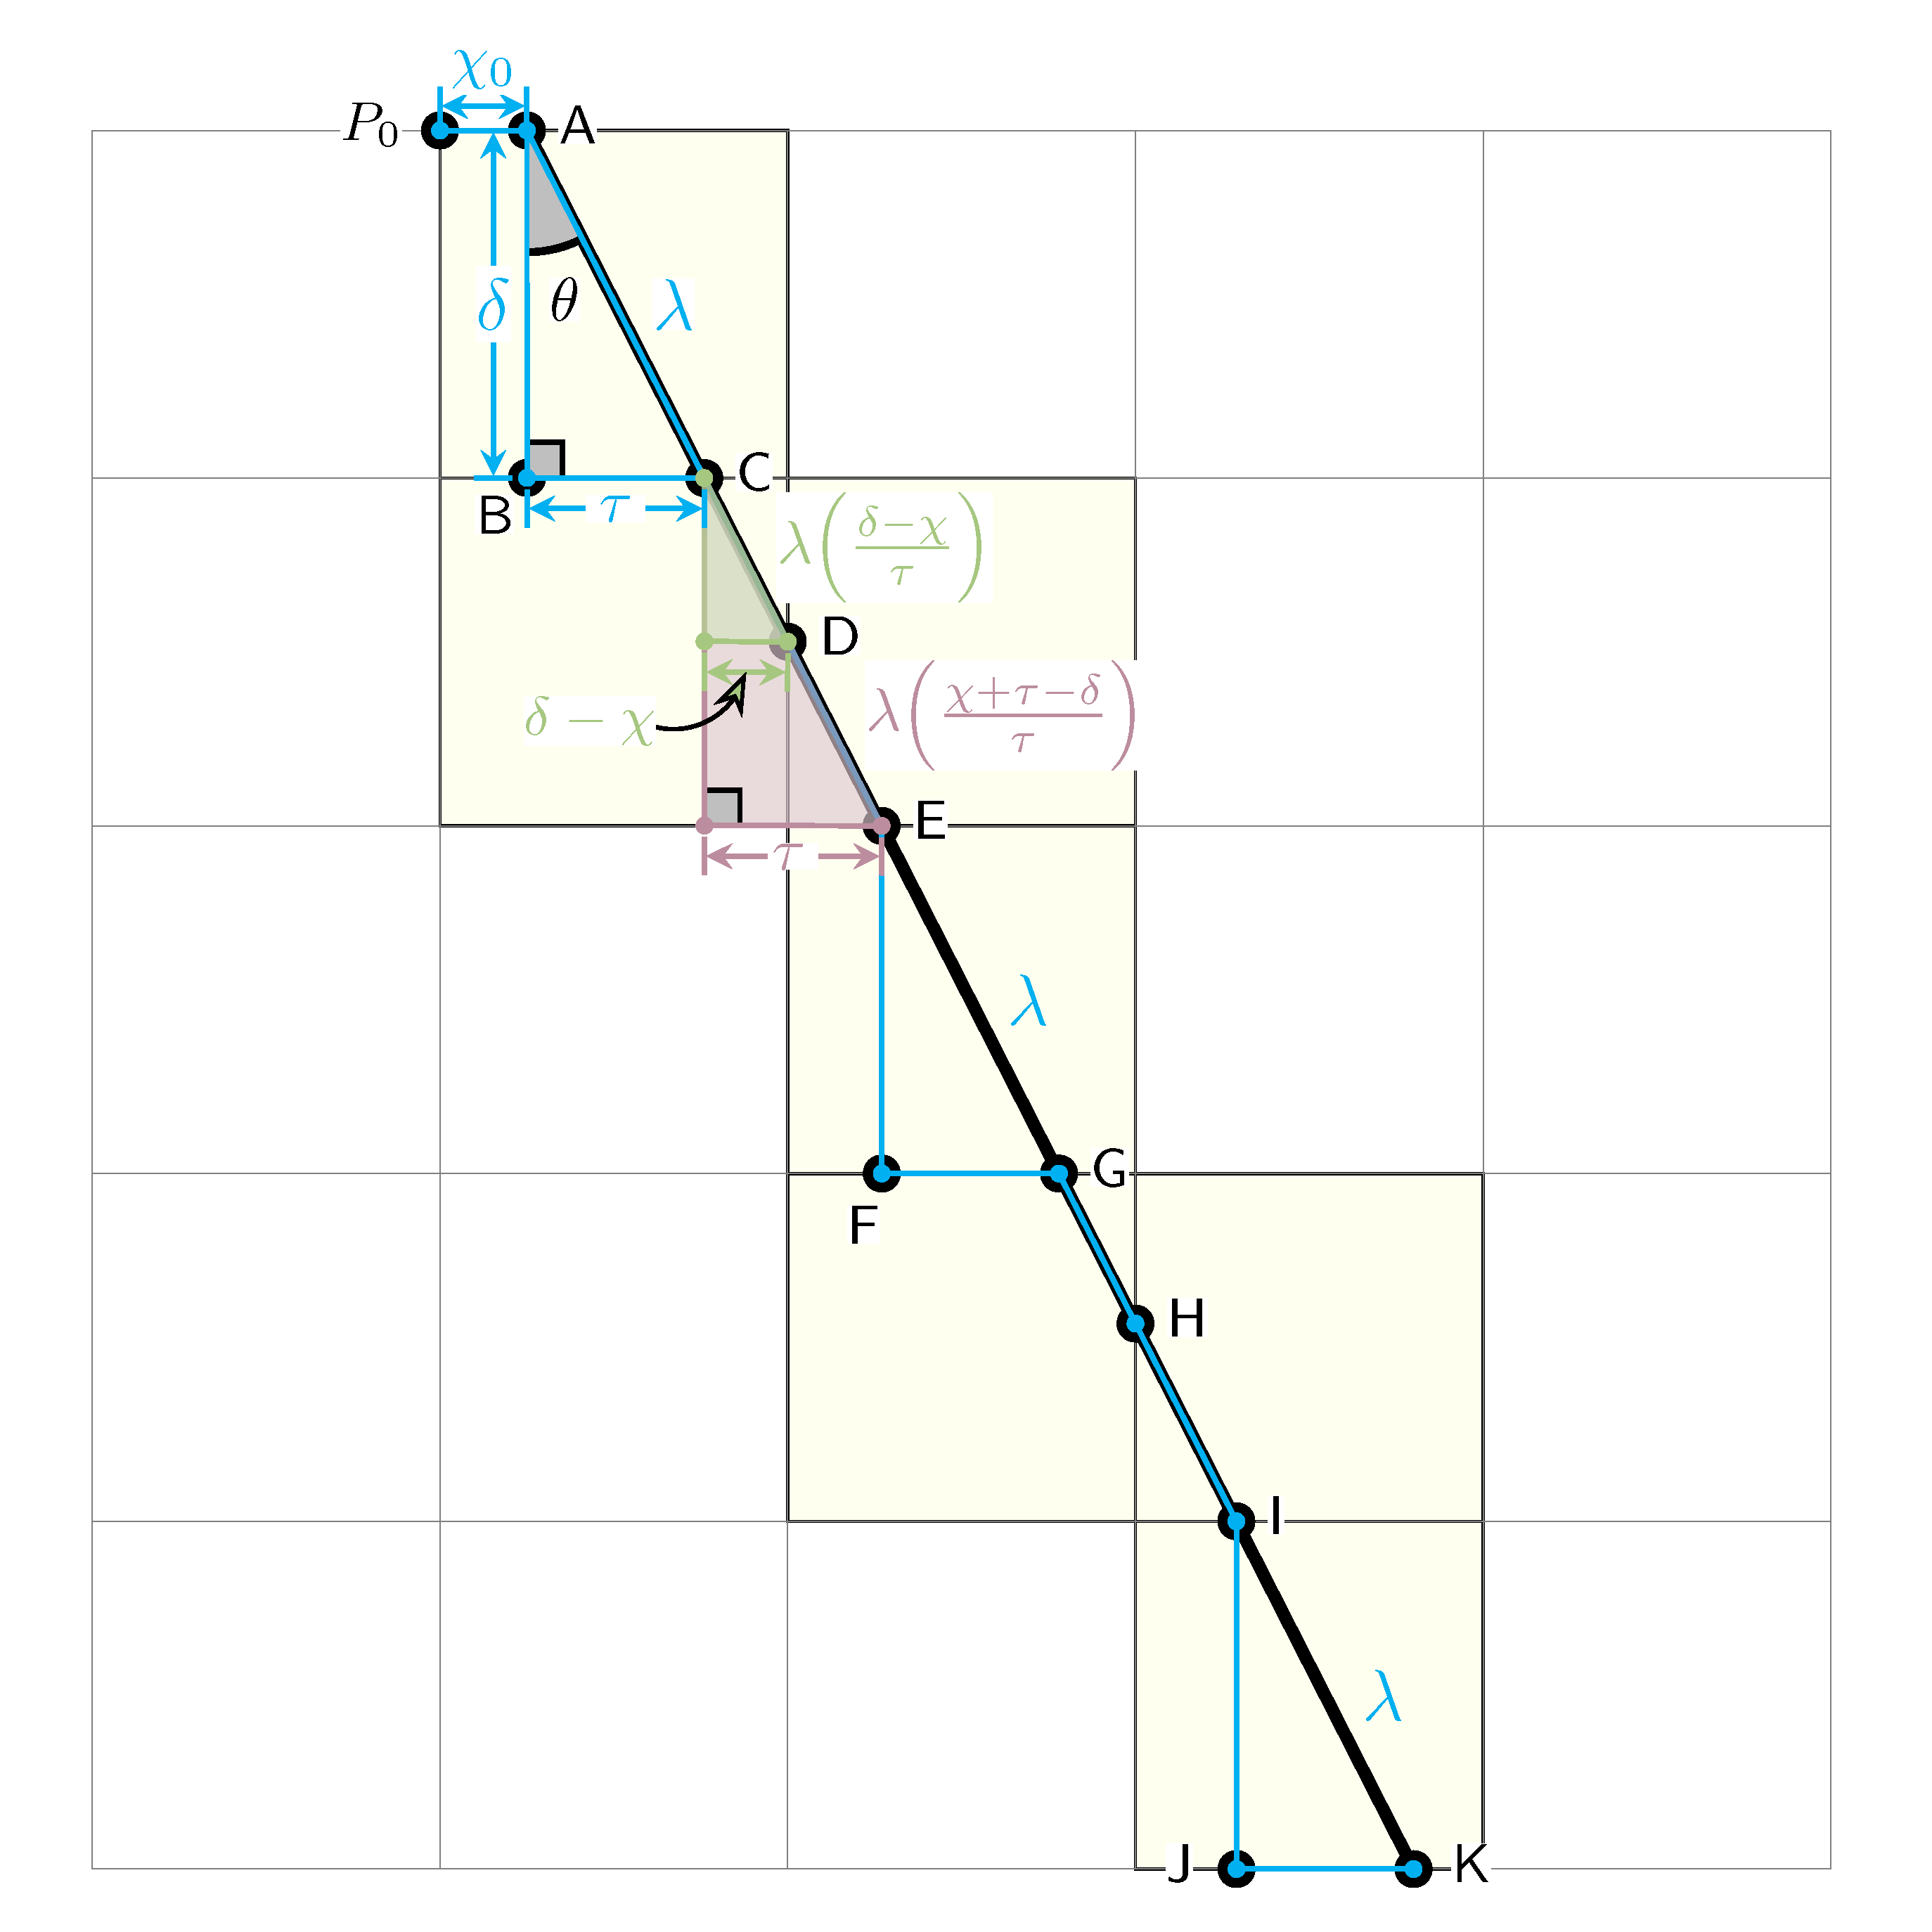
\includegraphics[width=4cm]{DDA.png}
    \caption{Hello DDA figure caption}\label{fig:DDA}
\end{figure}
%_______________________________________________________________________________________________________________________________%
%*******************************************************************************************************************************%
%===============================================================================================================================%
%------------------------------------------------ END: C2-HistoricalReview.tex -------------------------------------------------%
%===============================================================================================================================%
%*******************************************************************************************************************************%
%_______________________________________________________________________________________________________________________________%
%-------------------------------------------------------------------------------------------------------------------------------%
\endinput

	
%------------------------------------------------------------------------------------------------------------------------------%
%_______________________________________________________________________________________________________________________________%
%*******************************************************************************************************************************%
%===============================================================================================================================%
%------------------------------------------------------- C3-Methods.tex --------------------------------------------------------%
%===============================================================================================================================%
%*******************************************************************************************************************************%
%_______________________________________________________________________________________________________________________________%
%-------------------------------------------------------------------------------------------------------------------------------%
\chapter{Methods}\label{chap:methods}

Present what you did and how. May be a single Methods Chapter, or separate Methods Sections if separate topics of your dissertation are each presented as individual chapters. Alternatively, if there are methods that are relevant to all your topics, as well as methods germane to each topic individually, there might be a separate Methods Chapter here as well as Methods Sections in each topical Chapter. Cite your work where applicable~\cite{AuthorYear}.

\textbf{NOTE:} This may be broken into two chapters, e.g. '\textbf{Materials}' and '\textbf{Methods}'
%_______________________________________________________________________________________________________________________________%
%*******************************************************************************************************************************%
%===============================================================================================================================%
%----------------------------------------------------- END: C3-Methods.tex -----------------------------------------------------%
%===============================================================================================================================%
%*******************************************************************************************************************************%
%_______________________________________________________________________________________________________________________________%
%-------------------------------------------------------------------------------------------------------------------------------%
\endinput


\subappendix{Notation and glossary}{
%\begin{subappendices}
    \label{app:glossary-notation}
    \input{C3-A-Defs}
%\end{subappendices}
}
%------------------------------------------------------------------------------------------------------------------------------%
\include{C4-HullDetection}

\subappendix{Voxel Walk Algorithm}{
%\begin{subappendices}
    \input{C4-A-3D-DDA}
%\end{subappendices}
}
%------------------------------------------------------------------------------------------------------------------------------%
%\clearpage
%------------------------------------------------------------------------------------------------------------------------------%
\include{C5-MLP}

\subappendix{Derivation of simplified MLP}{
%\begin{subappendices}
    \input{C5-A-MLP}
%\end{subappendices}
}
%------------------------------------------------------------------------------------------------------------------------------%
\clearpage
%------------------------------------------------------------------------------------------------------------------------------%
%\input{Resubmission_clean.tex}

\include{C6-NTVS}

%------------------------------------------------------------------------------------------------------------------------------%
%\include{C7-Summary}
\include{C7-Conclusion}

%------------------------------------------------------------------------------------------------------------------------------%
%%-------------------------------------------------------------------------------------------------------------------------------%
%*******************************************************************************************************************************%
%******************************************************** C1-Intro.tex *********************************************************%
%*******************************************************************************************************************************%
%-------------------------------------------------------------------------------------------------------------------------------%
\chapter[Intro]{Introduction (Level 2)}\label{chap:intro}

Overview of dissertation: motivation, the reason more work is needed, the importance of your work and how it addresses this need, and a topical overview of what will be presented in the following chapters.

\section{First section (Level 3)}

Some first section text
\subsection{First subsection (Level 4) of First Section (Level 3)}

Some first subsection text
\subsubsection{First subsubsection (Level 5) of First Subsection (Level 4)}

Some first subsubsection text
\section{Second Section (Level 3)}
\subsection{First subsection (Level 4) of Second Section (Level 3)}
\subsubsection{First subsubsection (Level 5) of Second Subsection (Level 4)}
\section*{Third section (Level 3): unnumbered \textbackslash section* variant}
%
This section appears in the main document body here but \textbackslash section* (1) generates an UNNUMBERED section heading
and (2) DOES NOT create a corresponding ToC list item.

The same behavior is true for \textbackslash subsection* and \textbackslash subsubsection*.
%-------------------------------------------------------------------------------------------------------------------------------%
%*******************************************************************************************************************************%
%******************************************************** C1-Intro.tex *********************************************************%
%*******************************************************************************************************************************%
%-------------------------------------------------------------------------------------------------------------------------------%
\endinput 
%
%%_______________________________________________________________________________________________________________________________%
%*******************************************************************************************************************************%
%===============================================================================================================================%
%--------------------------------------------------- C2-HistoricalReview.tex ---------------------------------------------------%
%===============================================================================================================================%
%*******************************************************************************************************************************%
%_______________________________________________________________________________________________________________________________%
%-------------------------------------------------------------------------------------------------------------------------------%
\chapter{Historical Review and Literature Survey}\label{chap:history}

Present history of the research in your field/topic and an overview of the published literature relevant to this work. Prove that you are knowledgable about the existing literature in your field/topic so you can show why what you have done truly is new and important and represents a worthwhile contribution to the advancement of this field/topic.

\textbf{NOTE:} This may be broken into two chapters.
\begin{figure}
    \centering
    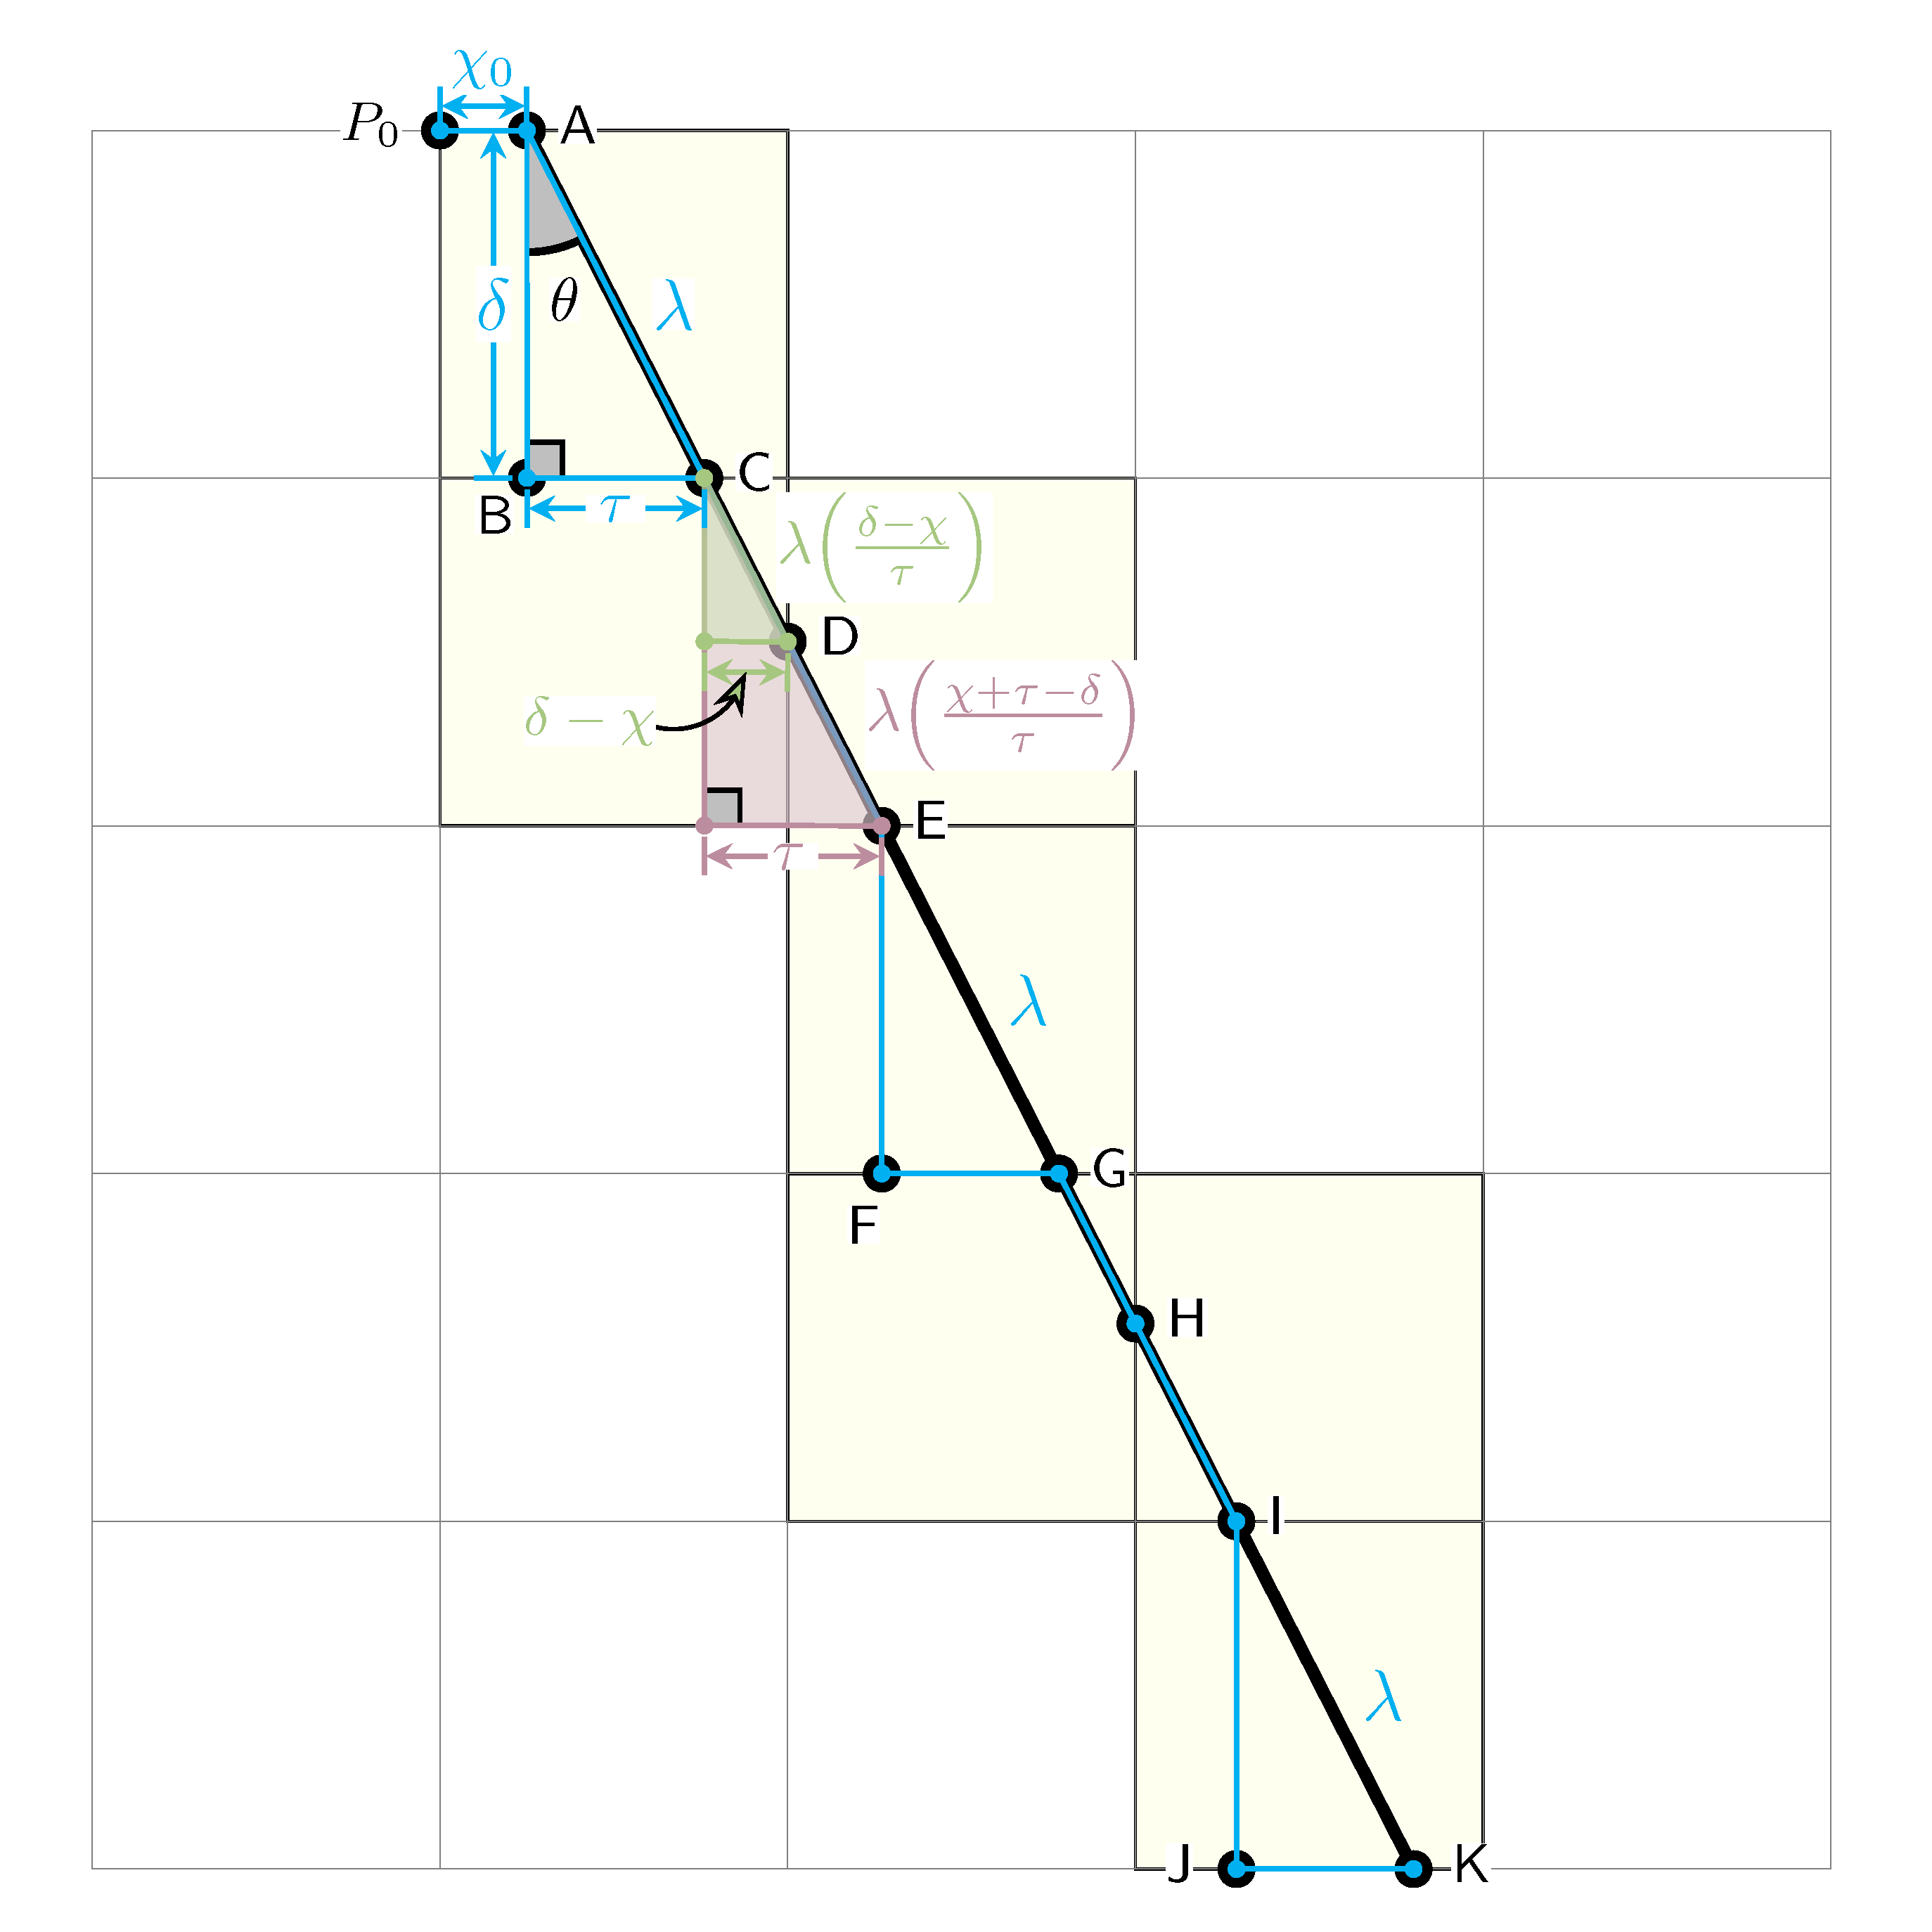
\includegraphics[width=4cm]{DDA.png}
    \caption{Hello DDA figure caption}\label{fig:DDA}
\end{figure}
%_______________________________________________________________________________________________________________________________%
%*******************************************************************************************************************************%
%===============================================================================================================================%
%------------------------------------------------ END: C2-HistoricalReview.tex -------------------------------------------------%
%===============================================================================================================================%
%*******************************************************************************************************************************%
%_______________________________________________________________________________________________________________________________%
%-------------------------------------------------------------------------------------------------------------------------------%
\endinput

%	
%%_______________________________________________________________________________________________________________________________%
%*******************************************************************************************************************************%
%===============================================================================================================================%
%------------------------------------------------------- C3-Methods.tex --------------------------------------------------------%
%===============================================================================================================================%
%*******************************************************************************************************************************%
%_______________________________________________________________________________________________________________________________%
%-------------------------------------------------------------------------------------------------------------------------------%
\chapter{Methods}\label{chap:methods}

Present what you did and how. May be a single Methods Chapter, or separate Methods Sections if separate topics of your dissertation are each presented as individual chapters. Alternatively, if there are methods that are relevant to all your topics, as well as methods germane to each topic individually, there might be a separate Methods Chapter here as well as Methods Sections in each topical Chapter. Cite your work where applicable~\cite{AuthorYear}.

\textbf{NOTE:} This may be broken into two chapters, e.g. '\textbf{Materials}' and '\textbf{Methods}'
%_______________________________________________________________________________________________________________________________%
%*******************************************************************************************************************************%
%===============================================================================================================================%
%----------------------------------------------------- END: C3-Methods.tex -----------------------------------------------------%
%===============================================================================================================================%
%*******************************************************************************************************************************%
%_______________________________________________________________________________________________________________________________%
%-------------------------------------------------------------------------------------------------------------------------------%
\endinput

%
%%%_______________________________________________________________________________________________________________________________%
%*******************************************************************************************************************************%
%===============================================================================================================================%
%------------------------------------------------------- C4-Results.tex --------------------------------------------------------%
%===============================================================================================================================%
%*******************************************************************************************************************************%
%_______________________________________________________________________________________________________________________________%
%-------------------------------------------------------------------------------------------------------------------------------%
\chapter{Results}\label{chap:results}

Present the results generated using the new methods you have developed and presented here. Again, you may choose to forego a Results Chapter in favor of presenting Results Sections when individual topics of your dissertation are provided as separate chapters. In such cases, you will likely have Methods, Results and potentially Summary/Conclusion Sections in each chapter.

It is theoretically possible you may not only have Methods that are applicable to every presented (chapter) topic, but you may also have results that are applicable to every presented (chapter) topic. In that case, you could have separate Methods/Results Chapters as well as Methods/Results Sections in each Topical Chapter; the order in which the Results Chapter is included in this scenario depends on the particular scenario.

%_______________________________________________________________________________________________________________________________%
%*******************************************************************************************************************************%
%===============================================================================================================================%
%----------------------------------------------------- END: C4-Results.tex -----------------------------------------------------%
%===============================================================================================================================%
%*******************************************************************************************************************************%
%_______________________________________________________________________________________________________________________________%
%-------------------------------------------------------------------------------------------------------------------------------%
\endinput


%
%%-------------------------------------------------------------------------------------------------------------------------------%
%*******************************************************************************************************************************%
%******************************************************* C5-Summary.tex ********************************************************%
%*******************************************************************************************************************************%
%-------------------------------------------------------------------------------------------------------------------------------%
\chapter{Summary}\label{chap:summary}

Summarize and discuss results from each topic and their collective impact/importance on the field/topic. Alternatively, the summary may be combined with the conclusions to form a single Conclusion chapter.
%-------------------------------------------------------------------------------------------------------------------------------%
%*******************************************************************************************************************************%
%************************************************* END OF FILE: C5-Summary.tex *************************************************%
%*******************************************************************************************************************************%
%-------------------------------------------------------------------------------------------------------------------------------%
\endinput


%-------------------------------------------------------------------------------------------------------------------------------%
%*******************************************************************************************************************************%
%****************************************************** BACKMATTER CONTENT *****************************************************%
%*******************************************************************************************************************************%
%-------------------------------------------------------------------------------------------------------------------------------%
%\include{Dissertation-Appendix}
%-------------------------------------------------------------------------------------------------------------------------------%
\bibliographystyle{IEEEtran}
\bibliography{authors,journal-names,IEEEfull,pct}								% Full journal names
%\bibliography{authors,journal-abrvs,IEEEabrv,pct}								% Abbreviated Journal names
%-------------------------------------------------------------------------------------------------------------------------------%
\end{document}
%-------------------------------------------------------------------------------------------------------------------------------%
%*******************************************************************************************************************************%
%************************************************ END: Dissertation-Schultze.tex ***********************************************%
%*******************************************************************************************************************************%
%-------------------------------------------------------------------------------------------------------------------------------%
